%%%%%%%%%%%%%%%%%%%%%%%%%%%%%%%%%%%%%%%%%
% a0poster Landscape Poster
% LaTeX Template
%%%%%%%%%%%%%%%%%%%%%%%%%%%%%%%%%%%%%%%%%

\documentclass[a0,landscape]{a0poster}

\usepackage{multicol}
\usepackage[svgnames]{xcolor}
\usepackage{times} 
\usepackage{graphicx}
\usepackage{booktabs}
\usepackage[font=small,labelfont=bf]{caption}
\usepackage{amsfonts, amsmath, amsthm, amssymb}
\usepackage{wrapfig}
\usepackage{setspace} 
\usepackage{tikz}
\usetikzlibrary{shapes.geometric, arrows.meta, positioning, fit, backgrounds}
\usepackage[most]{tcolorbox} % Para las cajas de colores de fondo

% Configuración de columnas
\columnsep=40pt
\columnseprule=1pt

% Definición de colores para el póster
\definecolor{UDBlue}{RGB}{25, 43, 88}
\definecolor{UDGold}{RGB}{218, 171, 15}
\definecolor{SectionColor}{RGB}{0, 68, 129}
\definecolor{ListingBg}{RGB}{240, 240, 240}

% --- CONFIGURACIÓN DE COLORES ---
\definecolor{UDBlue}{RGB}{25, 43, 88}
\definecolor{PastelBlue}{RGB}{230, 240, 255}   % Azul pastel para columnas laterales
\definecolor{PastelYellow}{RGB}{255, 253, 220} % Amarillo pastel para columna central
\definecolor{UDGold}{RGB}{218, 171, 15}

% --- ESTILO DE LAS SECCIONES (CAJAS) ---
\newtcolorbox{SeccionAzul}[1]{
    colback=PastelBlue, colframe=UDBlue, fonttitle=\bfseries\Huge, 
    title=#1, coltitle=white, sharp corners=south, boxrule=2pt, arc=10pt,
    before skip=1cm, after skip=1cm, left=1cm, right=1cm, top=1cm, bottom=1cm
}

\newtcolorbox{SeccionAmarilla}[1]{
    colback=PastelYellow, colframe=UDGold, fonttitle=\bfseries\Huge, 
    title=#1, coltitle=UDBlue, sharp corners=south, boxrule=2pt, arc=10pt,
    before skip=1cm, after skip=1cm, left=1cm, right=1cm, top=1cm, bottom=1cm
}

\renewcommand{\normalsize}{\fontsize{34}{40}\selectfont}
\begin{document}

%----------------------------------------------------------------------------------------
%   HEADER
%----------------------------------------------------------------------------------------

\begin{minipage}[b]{0.8\linewidth}
    \sffamily 
    \veryHuge \color{UDBlue} \textbf{Smart Energy Management System: A Systems Analysis and Design Approach} \color{Black}\\[0.5cm]
    \Huge\textit{Omar Y. Fonseca Lopez, Daniel F. Barrera Suarez, Daniel M. Ballesteros Molina, Dania L. Guzman Triviño }\\[0.5cm]
    \Large Systems Engineering Program, Universidad Distrital Francisco José de Caldas, Bogotá, Colombia  \\
    \Large \texttt{\{oyfonsecal, dfbarreras, dmballesterosm, dlguzmant\}@udistrital.edu.co }
\end{minipage}
\begin{minipage}[b]{0.18\linewidth}
    \centering
    % Asegúrate de que la ruta a esta imagen sea correcta
    \includegraphics[width=18cm]{figures/Escudo_UD.png}
\end{minipage}

\vspace{1cm}

%----------------------------------------------------------------------------------------
%   CONTENT
%----------------------------------------------------------------------------------------

\begin{multicols}{3}
\begin{spacing}{1.2} 

%================================================
% ABSTRACT
%================================================
\section*{Abstract}
{\large This work addresses inefficient energy consumption in Engineering Faculty laboratories, characterized by prolonged equipment use in unoccupied spaces. A software-defined, decentralized solution is proposed to operate in user-space via autonomous agents. These agents monitor inactivity, generate deterrent alerts, and execute energy-saving actions without requiring administrative privileges or infrastructure modifications.}

%================================================
% INTRODUCTION
%================================================
\section*{Introduction}
{\large
Efficient energy management in university environments is crucial due to the economic and environmental impacts of electricity consumption. Human behavior acts as a determining factor in energy waste, creating a gap between policies and real practices.}
{\large
While traditional IoT sensor-based solutions seem ideal, the institutional context imposes severe restrictions: lack of administrative privileges, prohibition of private networks, and inability to deploy additional hardware. To overcome this, we propose a software-based approach utilizing autonomous agents that operate in the user-space.}

%================================================
% METHODOLOGY & ARCHITECTURE
%================================================
\section*{Methodology and Architecture}
{\large The methodology follows a systems analysis approach applied to a socio-technical problem.}

\subsection*{Systems Analysis}
{\large Initial diagnostics (surveys and direct observation) revealed that the main driver of energy waste is human forgetfulness. Feasibility studies completely ruled out IoT solutions due to institutional infrastructure lock-downs.}

\subsection*{Software-Defined Architecture}
{\large The core solution is a distributed system driven by autonomous agents.}
\begin{itemize}{\large 
    \item \textbf{User-Space Execution:} The agent runs without requiring system-level administrative installation.
    \item \textbf{Telemetry Collection:} Interacts with local OS APIs (e.g., ctypes, psutil) to measure real-time activity.
    \item \textbf{Cloud Integration:} Sends statuses to a MySQL DBaaS and triggers notifications via an external messaging API (Telegram).
    }
\end{itemize}


\centering
\resizebox{\columnwidth}{!}{%
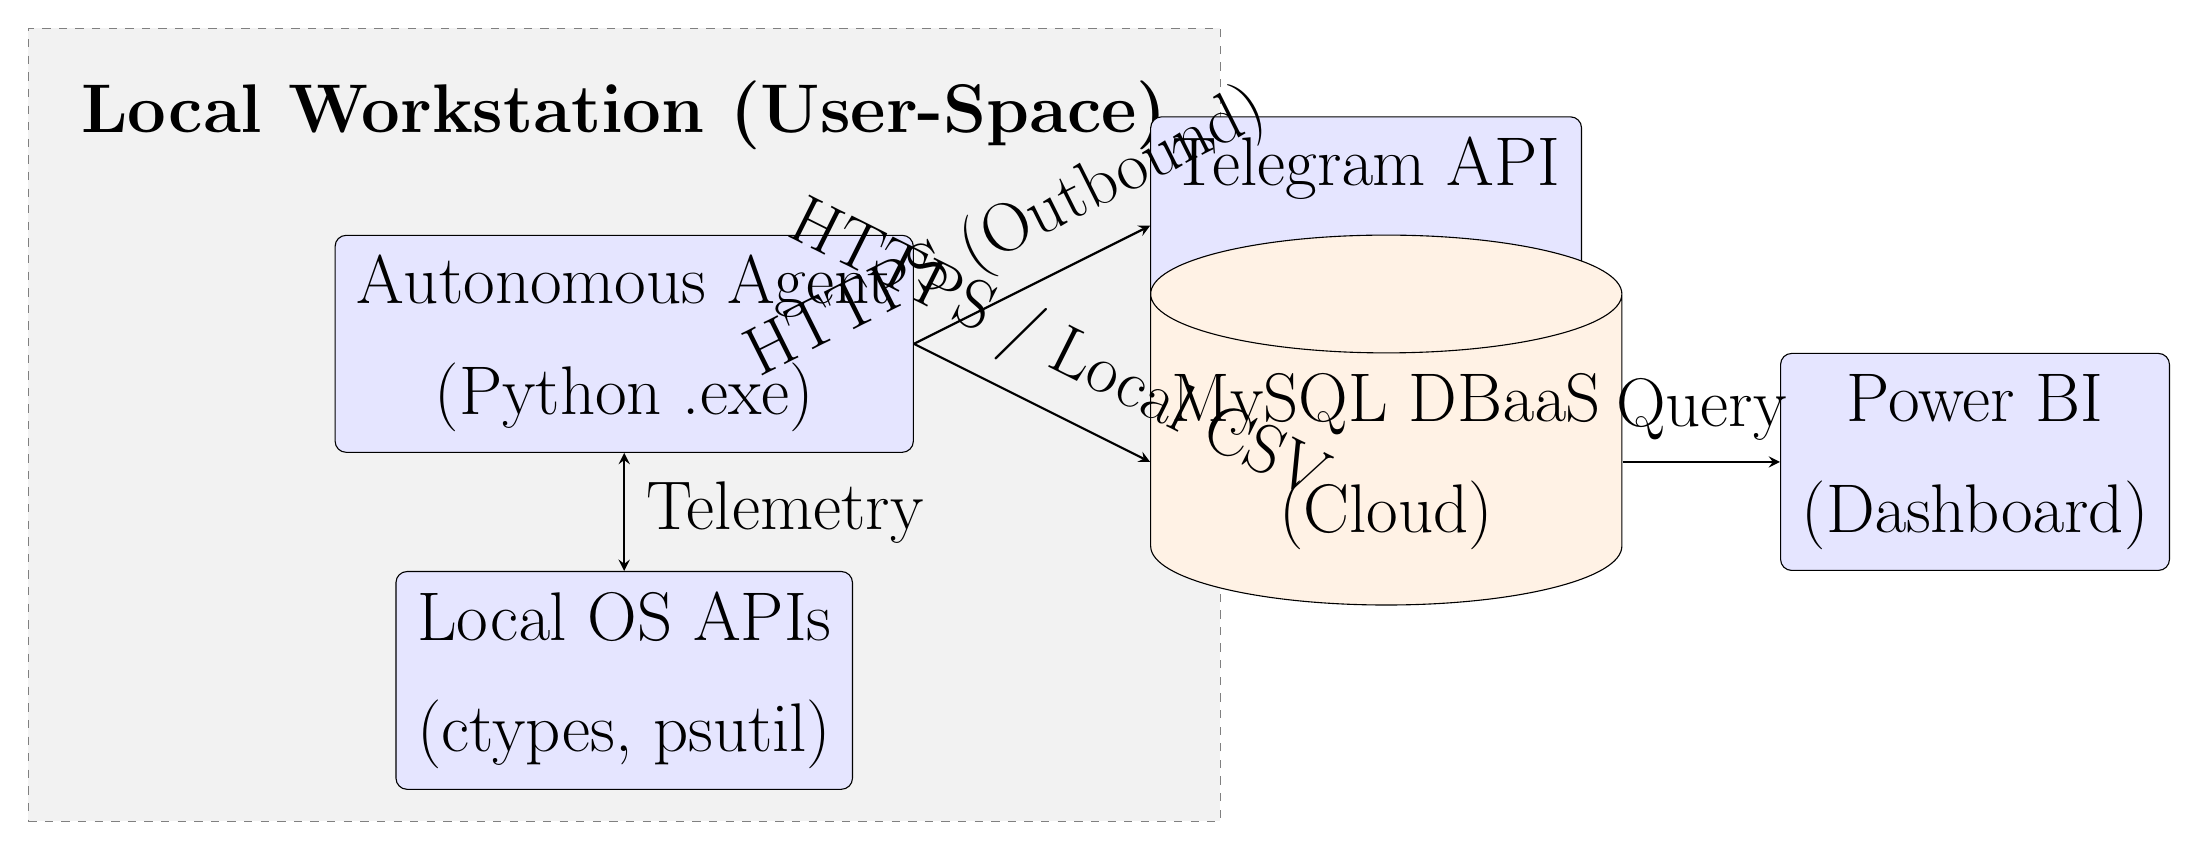
\begin{tikzpicture}[
    node distance=2cm and 3cm,
    box/.style={draw, rectangle, minimum width=3cm, minimum height=1.2cm, align=center, fill=blue!10, rounded corners},
    db/.style={draw, cylinder, shape border rotate=90, aspect=0.25, minimum height=1.5cm, minimum width=2.2cm, align=center, fill=orange!10},
    arrow/.style={->, >=stealth, thick}
]

\node[box] (agent) {Autonomous Agent \\ (Python .exe)};
\node[box, below=1.5cm of agent] (os) {Local OS APIs \\ (ctypes, psutil)};

\node[above=0.8cm of agent] (title) {\textbf{Local Workstation (User-Space)}};

\begin{scope}[on background layer]
    \node[fill=gray!10, draw=gray, dashed, fit=(title) (agent) (os), inner sep=0.4cm] (pc) {};
\end{scope}

\node[box, right=3cm of agent, yshift=1.5cm] (telegram) {Telegram API \\ (Alerts)};
\node[db, right=3cm of agent, yshift=-1.5cm] (mysql) {MySQL DBaaS \\ (Cloud)};
\node[box, right=2cm of mysql] (powerbi) {Power BI \\ (Dashboard)};

\draw[arrow, <->] (agent) -- node[right] {Telemetry} (os);
\draw[arrow] (agent.east) -- node[above, sloped] {HTTPS (Outbound)} (telegram.west);
\draw[arrow] (agent.east) -- node[above, sloped] {HTTPS / Local CSV} (mysql.west);
\draw[arrow] (mysql.east) -- node[above] {Query} (powerbi.west);

\end{tikzpicture}%
}

%================================================
% OPERATIONAL LOGIC
%================================================
\section*{Operational Logic}
{\large The autonomous agent implements a multi-stage intervention logic to ensure the user's data remains safe before taking action.}

{\large 
\begin{itemize}
  \item \textbf{Inactivity Loop:} Continuously verifies peripheral inactivity (mouse/keyboard).
  \item \textbf{CPU Verification:} If inactive for >15 minutes, it checks if the CPU load is under 20\% to avoid interrupting background tasks like rendering.
  \item \textbf{Nudge System:} Displays a 60-second visual warning. If not canceled by the user, it forces a secure OS suspension.
\end{itemize}}

\centering
\resizebox{\columnwidth}{!}{%
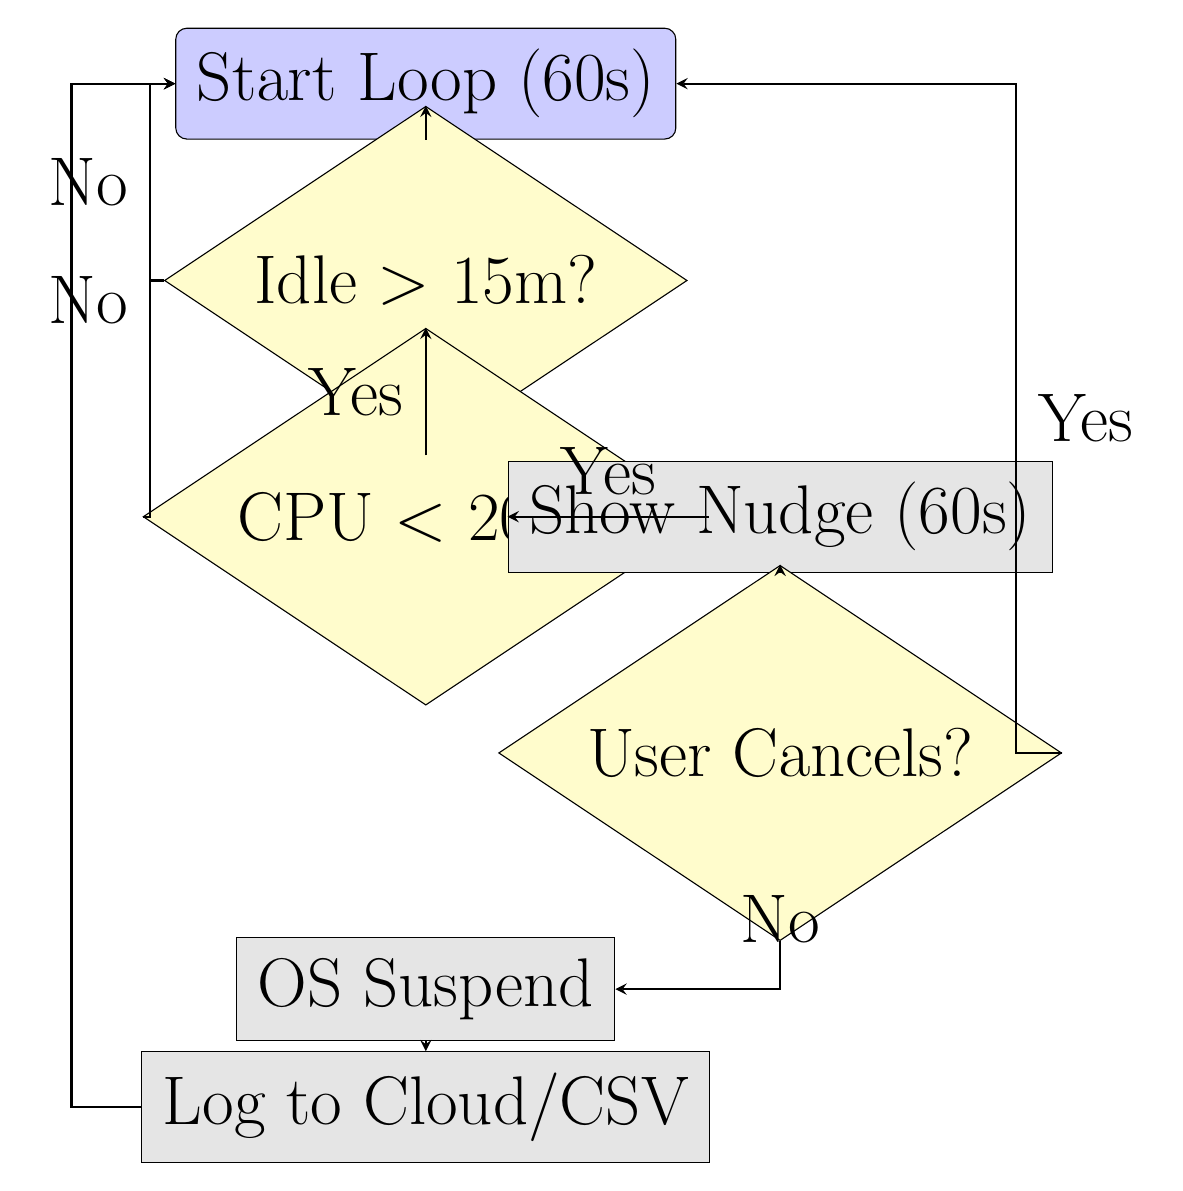
\begin{tikzpicture}[
    node distance=1.5cm,
    startstop/.style={rectangle, rounded corners, minimum width=2.5cm, minimum height=0.8cm, text centered, draw=black, fill=blue!20},
    process/.style={rectangle, minimum width=2.5cm, minimum height=0.8cm, text centered, draw=black, fill=gray!20},
    decision/.style={diamond, minimum width=2.5cm, minimum height=0.8cm, text centered, draw=black, fill=yellow!20, aspect=1.5},
    arrow/.style={thick,->,>=stealth}
]

\node (start) [startstop] {Start Loop (60s)};
\node (idle) [decision, below of=start, yshift=-1cm] {Idle $>$ 15m?};
\node (cpu) [decision, below of=idle, yshift=-1.5cm] {CPU $<$ 20\%?};
\node (nudge) [process, right of=cpu, xshift=3cm] {Show Nudge (60s)};
\node (cancel) [decision, below of=nudge, yshift=-1.5cm] {User Cancels?};
\node (suspend) [process, below of=cpu, yshift=-4.5cm] {OS Suspend};
\node (log) [process, below of=suspend] {Log to Cloud/CSV};

\draw [arrow] (start) -- (idle);
\draw [arrow] (idle) -- node[anchor=east] {Yes} (cpu);
\draw [arrow] (idle) -- ++(-3.5,0) |- node[anchor=east, near start] {No} (start);
\draw [arrow] (cpu) -- node[anchor=south] {Yes} (nudge);
\draw [arrow] (cpu) -- ++(-3.5,0) |- node[anchor=east, near start] {No} (start);
\draw [arrow] (nudge) -- (cancel);
\draw [arrow] (cancel) -- ++(3,0) |- node[anchor=west, near start] {Yes} (start);
\draw [arrow] (cancel) |- node[anchor=south, near start] {No} (suspend);
\draw [arrow] (suspend) -- (log);
\draw [arrow] (log) -- ++(-4.5,0) |- (start);

\end{tikzpicture}%
}


%================================================
% RESULTS & LIMITATIONS
%================================================
\section*{Expected Results}
{\large 
\begin{itemize}
    \item \textbf{Idle Time Reduction:} Measurable decrease in the time equipment remains powered on without usage.
    \item \textbf{Behavioral Mitigation:} Directly combats human negligence without needing physical IT hardware investments.
    \item \textbf{High Scalability:} Controlling energy from the User-Space is highly scalable for public institutions with blocked infrastructure.
\end{itemize}}

\subsection*{Limitations}
{\large The current Proof of Concept (PoC) faces specific constraints: }{\large 
\begin{itemize}
    \item \textbf{No Admin Rights:} Prevents the deployment of Windows Services or Active Directory GPOs.
    \item \textbf{Proxy Variables:} Lacking physical sensors, energy savings (kWh) are estimated mathematically via peripheral inactivity time.
    \item \textbf{Network Dependency:} Requires stable HTTPS outbound traffic for telemetry logging.
\end{itemize}}

%================================================
% CONCLUSION
%================================================
\section*{Conclusion}
{\large This project demonstrates that energy waste is deeply rooted in human behavioral dynamics rather than just technical flaws. By shifting the control intelligence from the physical infrastructure layer to the logical OS layer, it is possible to bypass severe institutional restrictions. This highly scalable approach sets a solid foundation for transitioning the university towards a "Smart Campus".}

%================================================
% REFERENCES
%================================================

{\large 
\begin{thebibliography}{99}
    \bibitem{doblari} M. V. Doblari, \textit{Gestión integral de energía en instituciones universitarias.} UNNOBA.
    \bibitem{abad} M. Abad Mier, \textit{Gestión energética de la biblioteca universitaria de la UVA, aplicando la ISO 50001.} 2015. 
    \bibitem{meza} B. Meza-Alcívar et al., \textit{Implementación de un sistema de gestión energético para institutos de educación superior.} 2023.
\end{thebibliography}}

\end{spacing}
\end{multicols}
\end{document}